\chapter{Analiza procesu}

W pierwszej kolejności przedstawiono ogólny opis procesu montażu płyt drukowanych oraz charakterystykę poszczególnych stanowisk.

\section{Ogólna charakterystyka}
Problem opisany w  niniejszej pracy dotyczy linii na której są montowane płyty drukowane do finalnych produktów.
Składa się on z następujących etapów:
\begin{enumerate}
	\item Pobranie potrzebnych elementów elektronicznych z magazynu.
	\item Uzbrojenie automatu pick\&place w wymagane elementy.
	\item Pobranie gotowych płyt PCB (ang. Printed Circuit Board).
	\item Ręczne nałożenie pasty lutowniczej za pomocą sitodruku.
	\item Uruchomienie procesu montażu elementów na maszynie pick\&place.
	\item Umieszczenie ręczne dodatkowych elementów (opcjonalnie).
	\item Przeprowadzenie procesu lutowania rozpływowego w piecu.
	\item Lutowanie ręczne (opcjonalnie).
	\item Kontrola gotowej płyty PCB\@.
\end{enumerate}

\breakparagraph{}
Specyfika procesu:
\begin{itemize}
	\item wszystkie procedury muszą być wykonane w ustalonej kolejności,
	\item proces wymaga operatorów,
	\item dla płyt dwustronnych należy powtórzyć sekwencję operacji,
	\item automat pick\&place może obsługiwać jednocześnie tylko jedną płytę PCB,
	\item piec lutowniczy może lutować jednocześnie kilka płyt drukowanych (liczba ta jest zależna od rozmiaru płyt).
\end{itemize}

Kompletny proces został przedstawiony przy pomocy diagramu na Rysunku~\ref{DiagFlow}.
Czerwone krawędzie wyznaczają ścieżkę krytyczną procesu.
Węzły o krawędziach przerywanych są to operacje opcjonalne, zależne od projektu płyty PCB\@.

\begin{figure}[H]
	\centering
	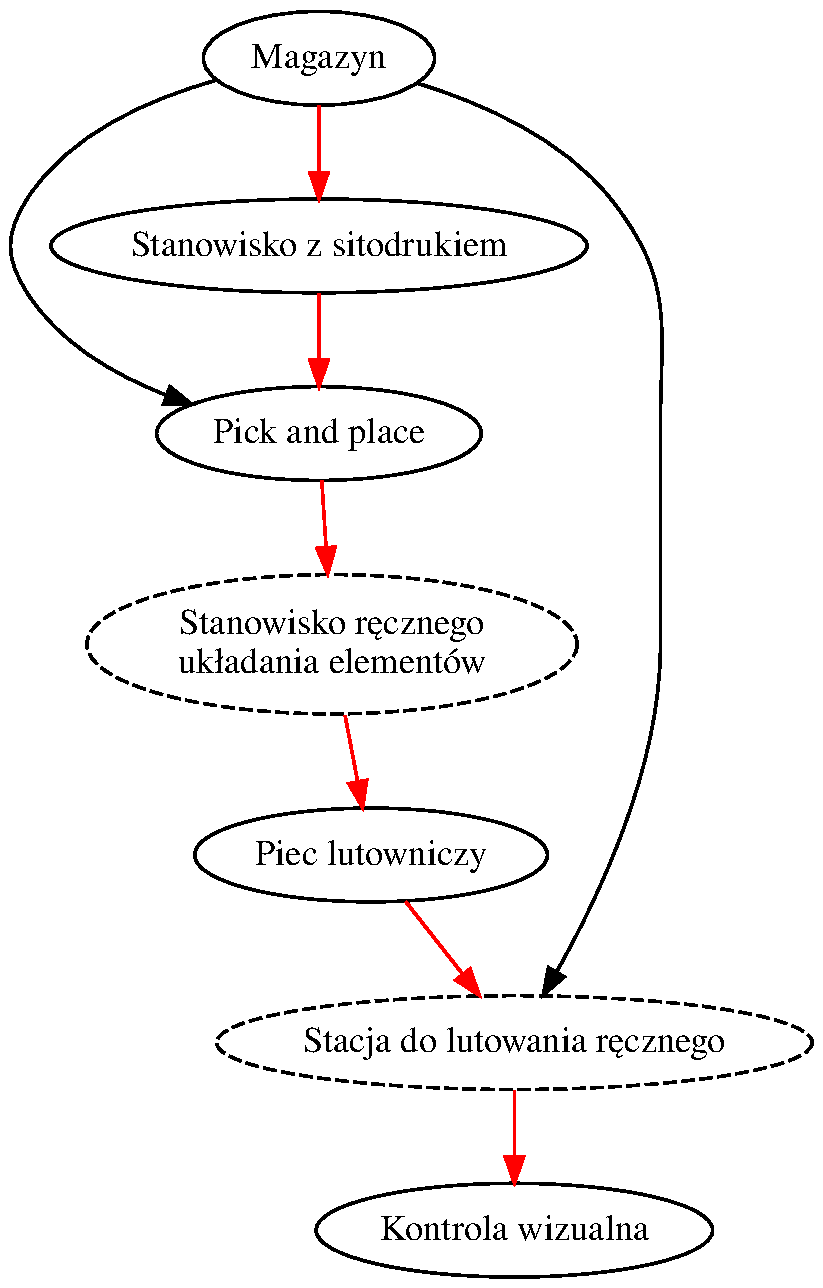
\includegraphics[scale=0.5]{./chapters/chapter2/flow_work.pdf}
	\caption{Diagram przepływu elementów w procesie}
	\label{DiagFlow}
\end{figure}

\section{Opis stanowisk}
W tej sekcji przedstawimy poszczególne stanowiska oraz pokrótce scharakteryzujemy.

\subsection{Magazyn}
Magazyn jest miejscem, od którego zaczyna się cały proces.
Przechowuje się w nim wszystkie niezbędne elementy elektroniczne (rezystory, kondensatory, układy scalone itd.), gotowe płyty PCB oraz szablony sitodruku dla poszczególnych projektów.
Aktualny stan magazynowy oraz fizyczna lokalizacja produktów znajduje się w bazie systemu ERP, który koordynuje dostawami elementów do stanowisk.
Wszystkie potrzebne elementy są pobierane bezpośrednio przez operatora.

\subsection{Stanowisko z sitodrukiem}
W kolejnym etapie produkcji gotowa płytka PCB tj. wytrawiony laminat z solder maską trafia na urządzenie sitodruku. Sitodruk jest to maszyna służąca do nakładania pasty lutowniczej wykorzystując szablon z wyciętymi miejscami na pola lutownicze.

\newpage{}
Maszyny te mogą pracować w kilku trybach~\cite{sitodruk}:
\begin{enumerate}
	\item Sitodruk manualny --- najprostsza wersja urządzenia. Cały proces sprowadza się do ręcznego ustawienia szablonu na płytce oraz ręcznego nałożenia pasty przez operatora. Cechuje się gorszą jakością i powtarzalnością operacji w porównaniu do urządzeń przedstawionych poniżej.
	\item Sitodruk półautomatyczny --- operator ustawia płytkę względem szablonu korzystając przy tym z odpowiedniego systemu wizyjnego. Proces naniesienia pasty odbywa się automatycznie. Rozwiązanie to jest często wykorzystywane przy prototypowaniu oraz produkcji małoseryjnej.
	\item Sitodruk automatyczny --- rola operatora sprowadza się do podania płytki i odebrania po naniesieniu pasty (tzw. system offline) lub załadowania podajnika czystymi płytkami a następnie odebraniu gotowych elementów (tzw. rozwiązanie in-line). Wszystkie czynności, takie jak ustawienie szablonu i nałożenie pasty, odbywają się automatycznie.
\end{enumerate}

W rozpatrywanym problemie jest stosowany sitodruk manualny (Rysunek~\ref{sitodruk}). Operator przed nałożeniem pasty na płytę PCB musi przezbroić maszynę. Sprowadza się to do pobrania szablonu z magazynu oraz ustawieniu go na tej maszynie. W następnym kroku następuje manualne naniesienie pasty.

\begin{figure}[H]
	\centering
	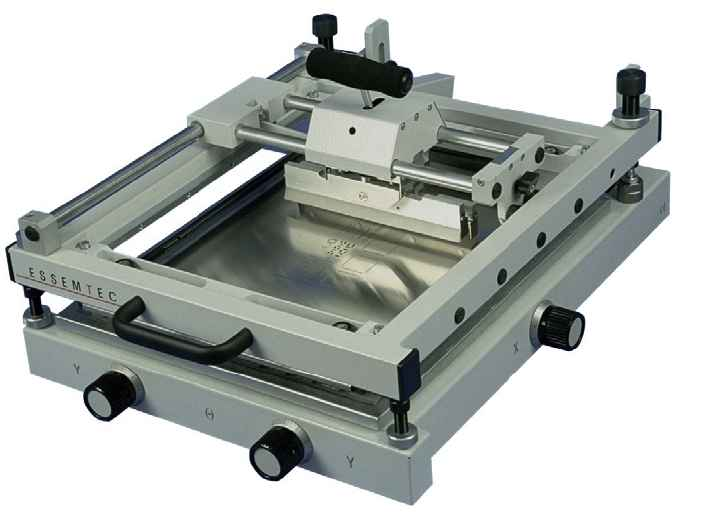
\includegraphics[scale=0.25]{./chapters/chapter2/sitodruk.jpg}
	\caption{Urządzenie sitodruku manualnego~\cite{sitodruk}.}
	\label{sitodruk}
\end{figure}

\newpage{}
\subsection{Automat pick\&place}
Automat pick and place jest to maszyna, która umożliwia w precyzyjny sposób układać komponenty SMD na płytkach PCB korzystając z odpowiedniego systemu wizyjnego~\cite{automatp&p1}. W rozpatrywanym procesie wykorzystywany jest automat M10V firmy Mechatronika (Rysunek~\ref{automat_pick_place}). Średnia wydajność maszyny to około 1200 --- 1600 komponentów na godzinę.

\breakparagraph{}
Maszynę tę cechuje~\cite{automatp&p2}:
\begin{itemize}
	\item wbudowany system wizyjny,
	\item pełna automatyzacja nanoszenia elementów na płytę drukowaną,
	\item automatyczna korekcja położenia na podstawie znaczników (ang.\ fiducials),
	\item korygowanie elementów na podstawie wykrycia złych oznaczeń na płycie,
	\item automatyczna zmiana dysz umożliwiająca nanoszenie różnej wielkości elementów ,
	\item automatyczne podawanie luźnych elementów (po wcześniejszej kalibracji),
	\item dane dotyczące projektów mogą pochodzić z różnych systemów danych CAD lub być wprowadzane ręcznie w trybie TEACH-IN\@.
\end{itemize}

Maszynę przed rozpoczęciem pracy z płytą PCB należy odpowiednio przezbroić. Operacja przezbrojenia polega na załadowaniu poszczególnych elementów elektronicznych oraz wykonaniu jej kalibracji.

\breakparagraph{}
Elementy mogą być dostarczane na kilka sposobów:
\begin{itemize}
	\item taśmy: 8 mm, 12 mm, 16 mm, 24 mm, 32 mm, 44 mm,
	\item tacki JEDEC --- opakowanie w kształcie matrycy w której są przechowywane układy scalone,
	\item tuby (ang. sticks) SO8–PLCC84 --- opakowanie antystatyczne w którym elementy są ułożone w lini,
	\item elementy luzem.
\end{itemize}

\begin{figure}[H]
	\centering
	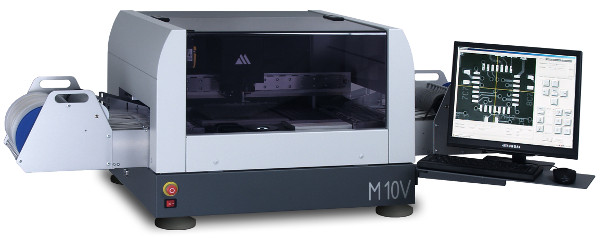
\includegraphics[scale=0.45]{./chapters/chapter2/M10V.jpeg}
	\caption{Automat M10V~\cite{automatp&p2}.}
	\label{automat_pick_place}
\end{figure}


\subsection{Piec lutowniczy}
Piec lutowniczy jest to urządzenie, które umożliwia zastosowanie techniki lutowania rozpływowego elementów SMD\@. Ważnym zagadnieniem przy lutowaniu rozpyłowym jest profil termiczny. Na podstawie profilu szacujemy czas trwania operacji w piecu.

\breakparagraph{}
Profil termiczny został schematycznie przedstawiony na Rysunku~\ref{schemat_termiczny} i składa się z następujących etapów:
\begin{description}
	\item[Etap 1:] Nagrzewanie wstępne (ang. preheat) --- wstępne nagrzewanie o jednostajnym wzroście temperatury w tempie 1--3\degree{C}, do osiągnięcia około 150\degree{C}. W tej fazie następuje częściowe odparowanie topnika.
	\item[Etap 2:] Oczyszczanie (ang. soak) --- aktywacja topnika umożliwiająca oczyszczenie chemiczne powierzchni złącza oraz usunięcie tlenków ze stopu lutowniczego. Etap ten trwa od 60 do 120 sekund.
	\item[Etap 3:] Jednostajne rozgrzanie do rozpływu (ang. ramp to peak) --- szybkie rozgrzanie mające na celu osiągnięcia temperatury likwidusu (temperatura przemiany ciała stałego w stan ciekły) stopu lutowniczego.
	\item[Etap 4:] Rozpływ (ang. reflow) --- faza zasadnicza lutowania rozpływowego. Zachodzi w temperaturze od 215 do 250\degree{C} (zależne od użytego stopu lutowniczego). Na tym etapie płynny stop tworzy połączenie pomiędzy polem lutowniczym, a elementem elektronicznym. Czas trwania rozpływu to od 30 do 300 sekund.
	\item[Etap 5:] Chłodzenie (ang. cooling) --- ostatni etap polegający na możliwe szybkim schłodzeniu o jednostajnym spadku 3--4\degree{C}. Zbyt gwałtowne schłodzenie może spowodować naprężenie termiczne, które są groźne dla lutujących elementów.
\end{description}

\begin{figure}[H]
	\centering
	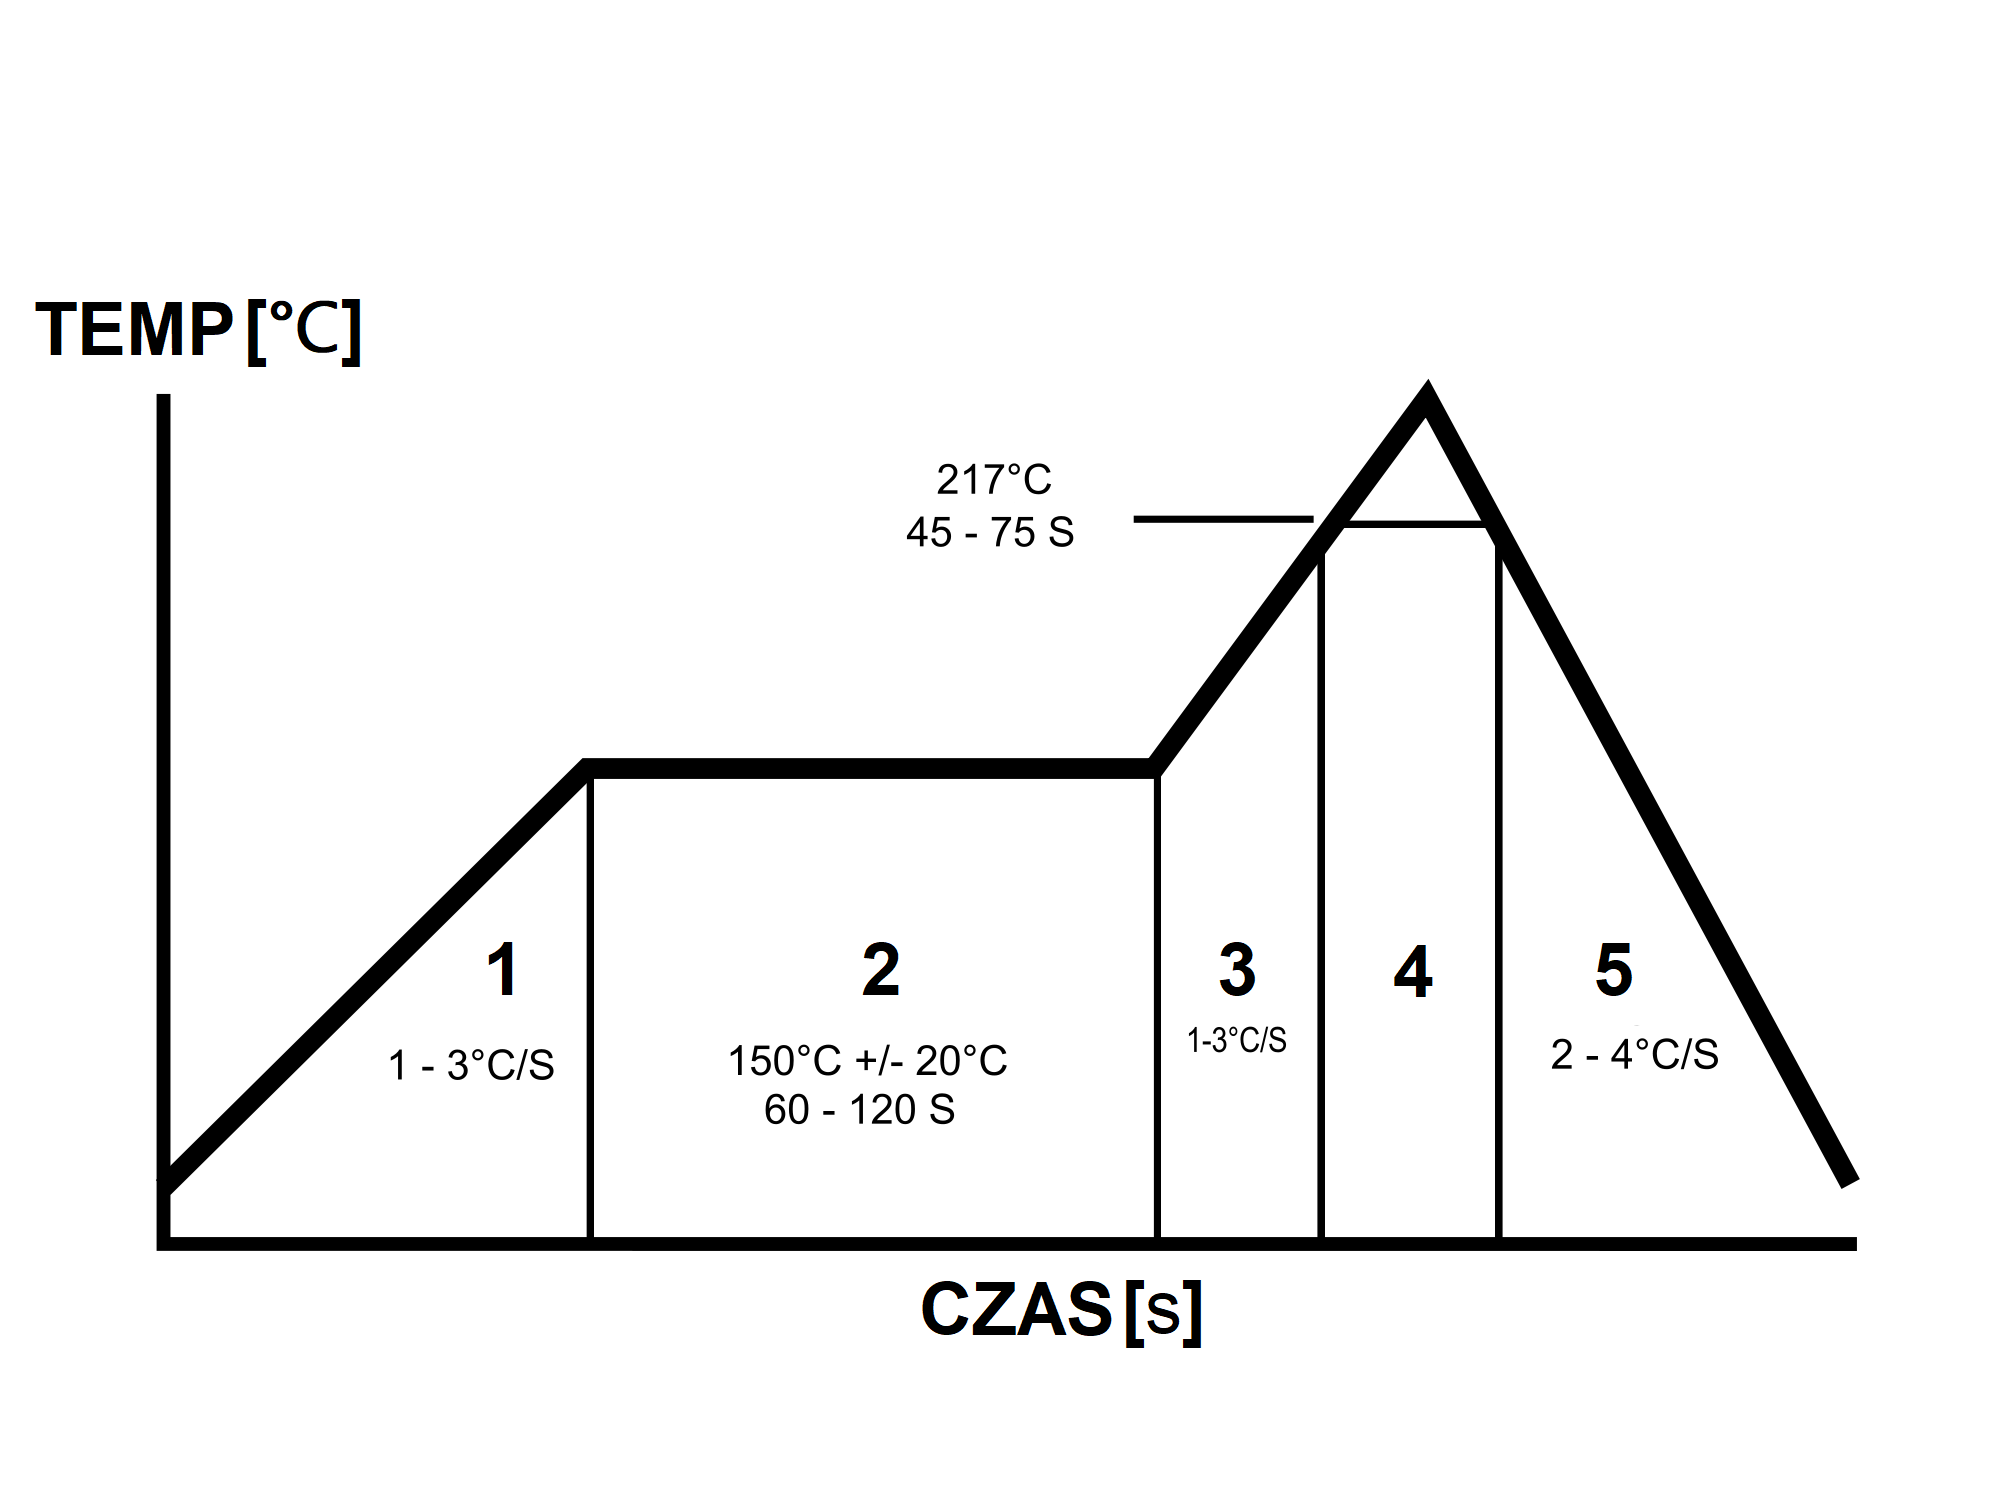
\includegraphics[scale=0.17]{./chapters/chapter2/schemat.png}
	\caption{Przebieg profilu termicznego w lutowaniu rozpływowym.}
	\label{schemat_termiczny}
\end{figure}

W rozpatrywanym procesie jest wykorzystywany piec eC-reflow-mate firmy Eurocircuits (Rysunek~\ref{piec}).


\begin{table}[H]
	\centering
	\caption{Specyfikacja pieca}
	\begin{tabular}{cc}
		\toprule
		Maksymalny rozmiar płyty PCB & 350 $\times$ 250 mm              \\\midrule
		Zakres temperatur             & Do 288 \degree{C}                \\\midrule
		Komunikacja z komputerem      & USB                              \\\midrule
		Wymiary                       & 520 $\times$ 620 $\times$ 245 mm \\\midrule
		Waga                          & około 25 kg                     \\
		\bottomrule
	\end{tabular}
\end{table}

\begin{figure}[H]
	\centering
	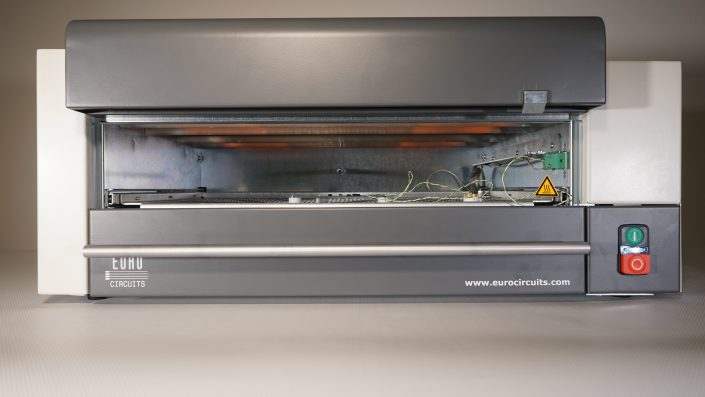
\includegraphics[scale=0.5]{./chapters/chapter2/piec.jpg}
	\caption{Piec lutowniczy eC-reflow-mate~\cite{piec}.}
	\label{piec}
\end{figure}

\subsection{Stanowisko do prac ręcznych}
Operacje przeprowadzane przez operatora na tym stanowisku polegają na nakładaniu i lutowaniu elementów oraz kontrolę wizyjną.

\breakparagraph{}
Stanowisko to jest wyposażone w następujący osprzęt:
\begin{itemize}
	\item stację lutowniczą,
	\item stację hot-air,
	\item narzędzia drobne (szczypce, pęsety itd.),
	\item uchwyty montażowe,
	\item mikroskop.
\end{itemize}

W bardziej zaawansowanych technologicznie procesach wytwarzania, wszystkie prace są wykonywane automatycznie.